\newpage
\section{Data}

% SECTIONS
% Experimental details
% Properties (preprocessing, cycles, confounding, …)
% Relevance; state-of-the-art
% Description of data subsets

\subsection{Data Source}

A biological dataset is used to evaluate the proposed methods. The DNA of a cell contains genes that are involved in many of the cell's functions. They are typically responsible for the production of a protein. The first step in this process is to copy its information to a Messenger RNA (mRNA) strand. To measure how active a specific gene is, we can measure how much of its mRNA we find in the cell.

Genes interact to fulfill a plethora of cell functions. For example, the expression of one gene might up- or down-regulate the expression of some other gene. This interaction is regulated by some biochemical process. 

For a variety of reasons, it is interesting to know how genes interact precisely, that is: what the regulatory network looks like. By jointly measuring the expression of a large set of mRNA strands we obtain an mRNA profile. Collecting a set of these profiles allows us to model the joint distribution of mRNA expression and the causal relations.

Specifically, we use mRNA profiles from \citet{kemmeren2014large}. They measured a profile of 6.182 genes in cells of the yeast species \textit{Saccharomyces cerevisiae} (baker's yeast), using DNA microarray technology (Figure \ref{fig:3:microarray}). The dataset consists of 262 observational samples obtained from unaltered wild type cells, and 1.484 interventional samples obtained from mutant cells where one gene was deactivated.

\begin{figure}[h]
    \centering
    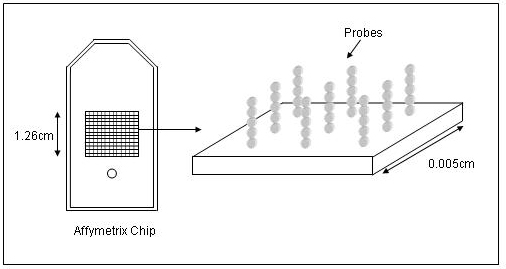
\includegraphics[width=.7\textwidth]{3microarray}
    \caption{Illustration of a typical microarray chip. Every small square can be used for an experiment to measure gene expression levels.\protect\footnotemark}
    \label{fig:3:microarray}
\end{figure}
\footnotetext{source: http://grf.lshtm.ac.uk/microarrayoverview.htm}

Both the observational and interventional profiles are reported relatively to some average wild type profile. \citet{kemmeren2014large} report that the interventional profiles are compared to a set of 428 wild type profiles. In this thesis, we work with the difference in $log_2$ fluorescent intensity, which indicates deviation from the normal gene expression levels.

% \silvan{It is unclear if the observational profiles are compared to the same set.} \silvan{ADD: measured as log2 fluorescent intensity} \silvan{ADD: some genes were excluded because they changed significantly in the WT already? see kemm. \textit{Statistical Analysis of Expression Profiles}}

There are some details of the experiments that might be of relevance in a discussion of underlying assumptions. First of all, the researchers chose to measure only a subset of about 25\% of all genes. Selection criteria included whether genes were expected to be involved in regulating other genes, and only genes were selected that do not play a vital role in keeping the cell alive (viability). 

Furthermore, the profile resulting from an experiment had to pass a quality control before being admitted to the dataset. Failing this test resulted either in repeating the experiment, or excluding the mutant. Although these checks improve the quality of the data by removing some failed experiments, they might also admit some selection bias. 

A final factor to consider is that  data from previous work of the same institute is included in the dataset, specifically from \citet{lenstra2011specificity} and \citet{van2010functional}. The authors note that they could not find any significant differences in the data. Nevertheless, this information can be seen as a context variable, and ignoring it is an explicit modelling assumption.

\subsection{Binary Ground-Truth}
We suppose that SCMs generate the dataset. Every gene expression is interpreted as an endogenous random variable. We suppose that there is an underlying causal mechanism (function $\B{f}$) that models the relations among these gene expressions. The interventional data is generated by a SCM induced by a perfect intervention on the expression of the mutant gene, making its expression a lot smaller. These interventions, along with the observational data, provide us with information about the SCM. 

The values in the interventional data represent deviations from the normal (wild-type) gene expressions that are measured when there is a perfect intervention on one gene (in the mutant). The more these values deviate from zero, the more likely it is that they are in fact deviating as a result of this intervention. We construct a set of binary ground-truth relations by selecting per intervened gene, those genes that respond with an absolute value exceeding some threshold. We interpret the result as a set of causes and (possibly indirect) effects. Two thresholds are used in this thesis. \citet{kemmeren2014large} used a threshold of $1.7$, stating that lower levels may be biologically relevant, but focussing on robust changes makes it more likely that they are biologically meaningful. We will also use this threshold, and introduce a lower one of $1.0$ which allows us to use more information of the system, and evaluate against a larger (but more noisy) set of ground-truth values. \silvan{Risk: high variance genes (why?), option: filter; why no other preprocessing? log2 diff is already something}

Often, we restrict ourselves to the 1.484 intervention genes (i.e. genes that occur in the intervention data as object of a perfect intervention) as possible effects, instead of all 6.182 measured genes. This makes it easier to interpret our metrics, because every relation between these genes is captured by the interventional data. We use the binary ground-truth to analyse the dataset, to inform our algorithm to find an order in the genes, and to evaluate causal methods. Scientific knowledge about some relations could be used to evaluate our methods as well, but it is incomplete and somewhat obscure because it is scattered about many papers with different experimental methods and conditions. 

\subsection{Properties}


Every intervention is a sample from an induced distribution, and there is little observational data, so we are dealing with sparsity. 

Partial correlation test supposes a normal distribution. How do genes differ in variance? How justified is this normality assumption?

Some methods including our order-based LCD assume acyclicity. Is this justified?

We should be aware of confounding. Why these alphas?


[DEADLINE 30 MINS EPIC FAST WRITING STUFF]



The validity of some of our modeling assumptions was tested using simple measurements on the dataset. We look at the sparsity of the data and the presence of cyclical relations and confounding. 

Binary ground-truth from interventional data, thresholds, filtering only intervened genes
(evt. why non-preprocessed: already ratio, different definitions very inconsistent)
(evt. option to filter high variance)

General properties
- variance, normality?, sparsity (one sample per 'interv. distr.')

cycles
- SCCs, length of simple? cycles?
- is order-based approach justified?

Confounding
- Not all confounding can be found by this simple method
- We make no causal sufficiency assumption, but: more confounding leaves less relations to be identified by LCD

\begin{figure}[h]
    \centering
    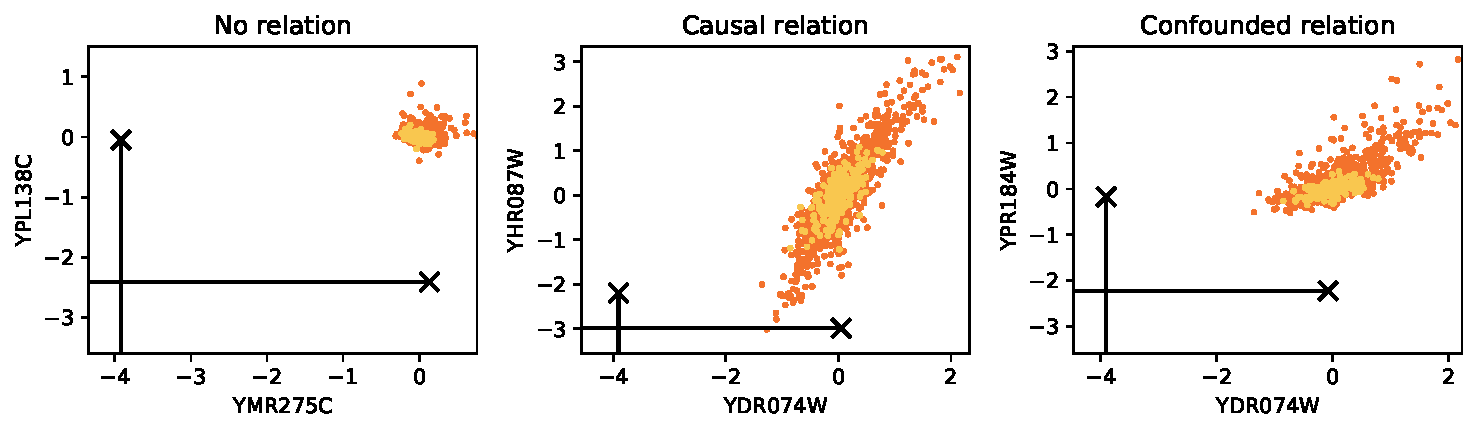
\includegraphics[width=\textwidth]{3gene_vs_gene}
    \caption{Gene VS gene}
    \label{fig:3:genevsgene}
\end{figure}

\begin{figure}[h]
    \centering
    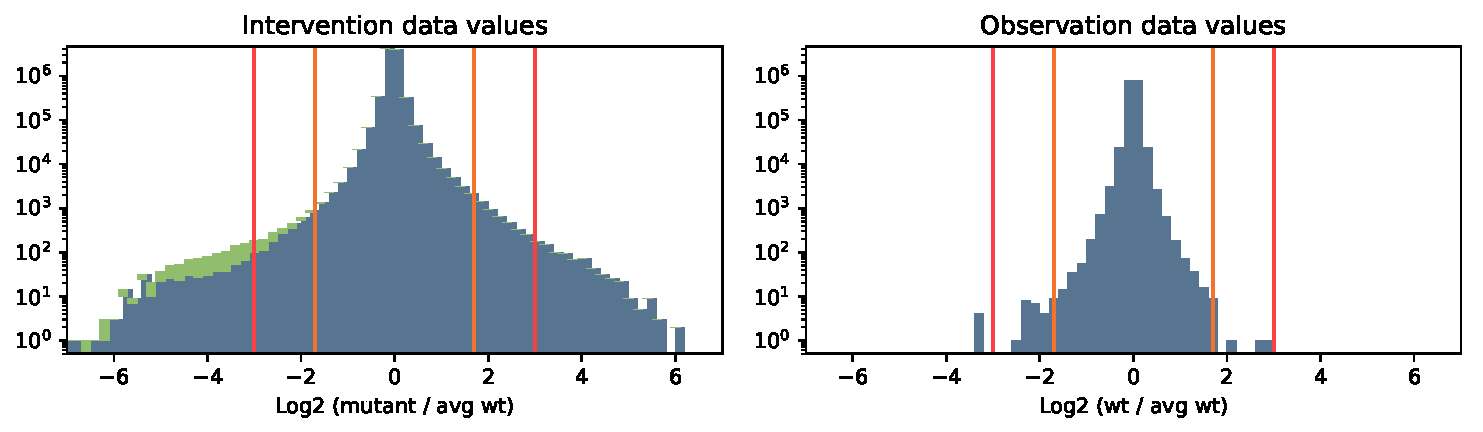
\includegraphics[width=\textwidth]{3data_values}
    \caption{Data values}
    \label{fig:3:datavalues}
\end{figure}

\begin{figure}[h]
    \centering
    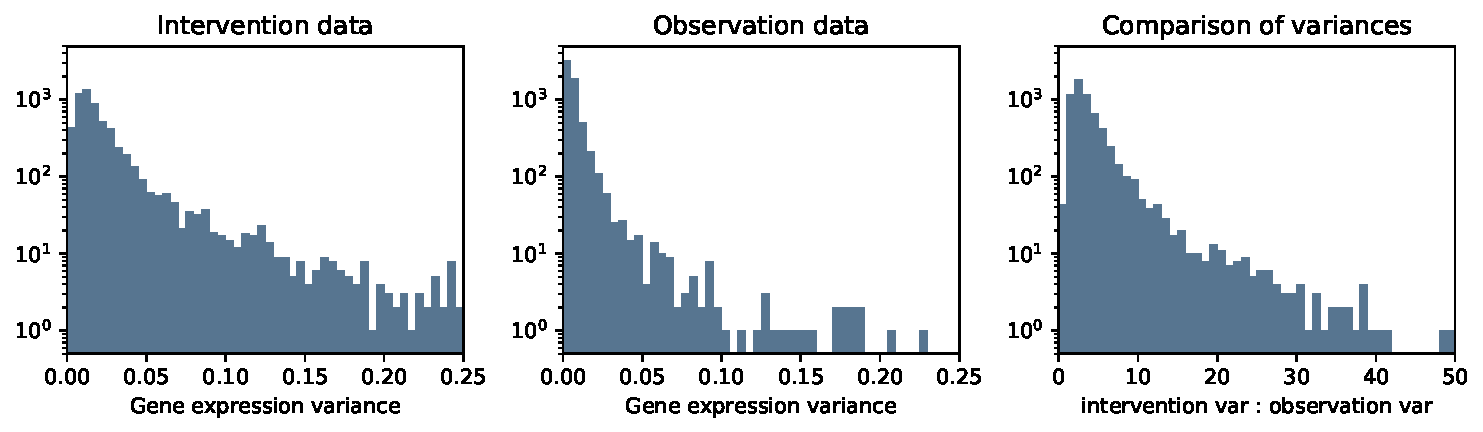
\includegraphics[width=\textwidth]{3gene_variance}
    \caption{Data variance}
    \label{fig:3:datavariance}
\end{figure}

\begin{figure}[h]
    \centering
    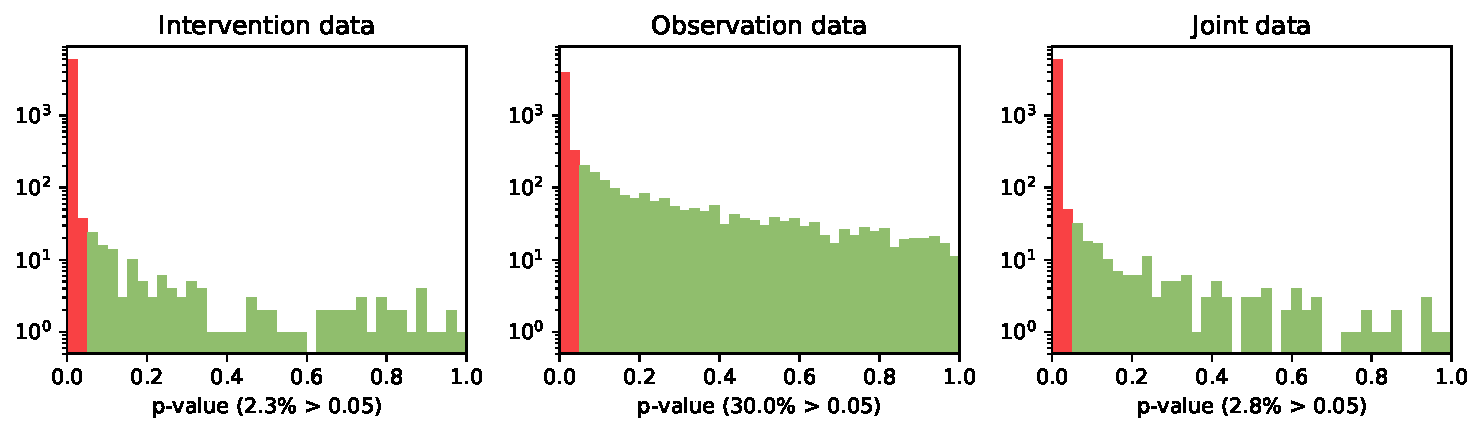
\includegraphics[width=\textwidth]{3normality}
    \caption{Gene normality}
    \label{fig:3:normality}
\end{figure}    

\begin{figure}[h]
    \centering
    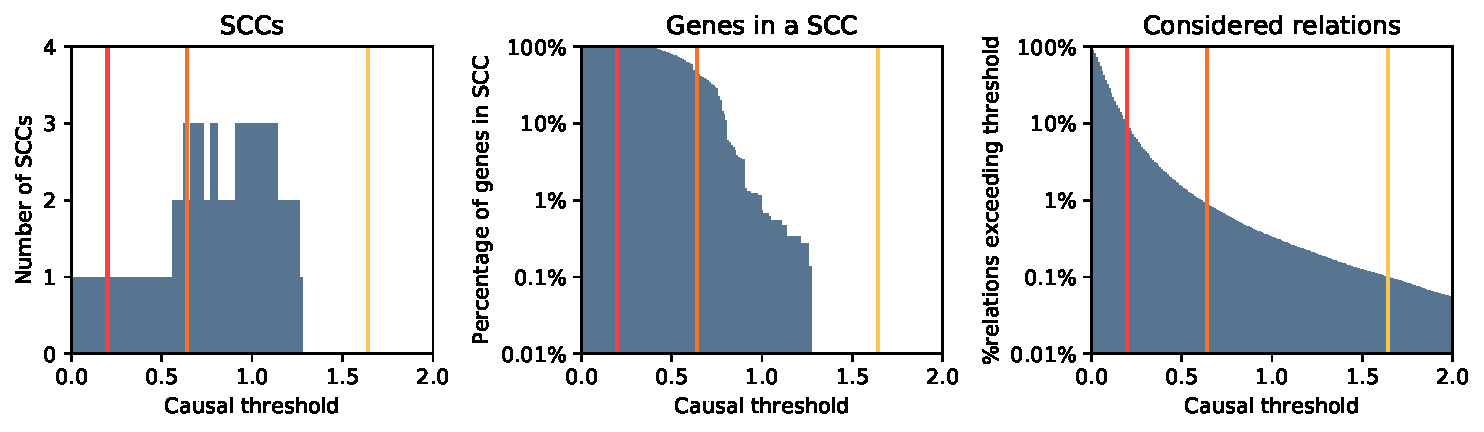
\includegraphics[width=\textwidth]{3cycles}
    \caption{Cycles}
    \label{fig:3:cycles}
\end{figure}    

\begin{figure}[h]
    \centering
    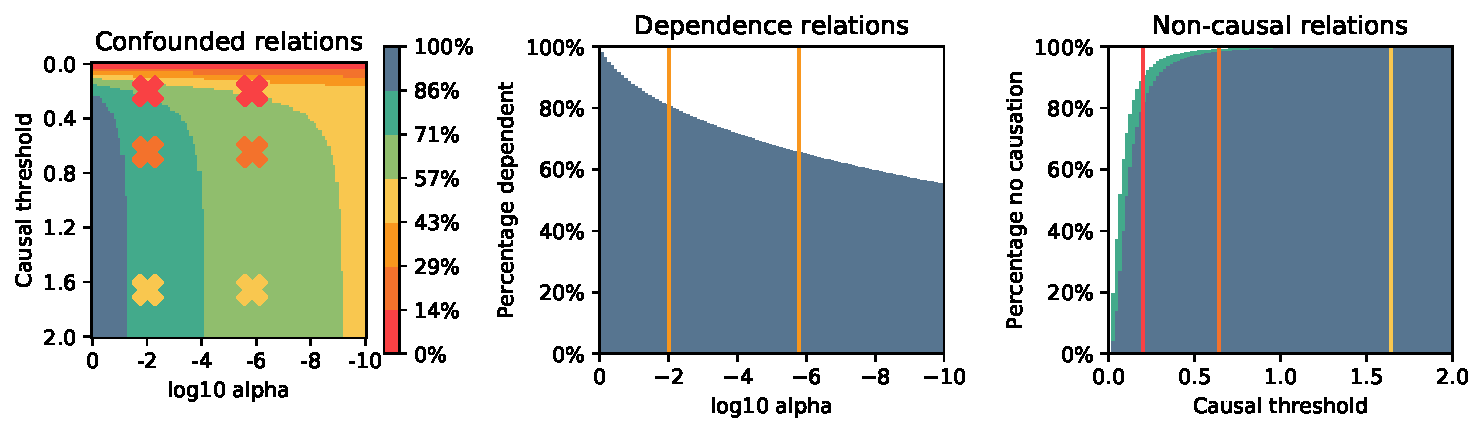
\includegraphics[width=\textwidth]{3confounding}
    \caption{Confounding}
    \label{fig:3:confounding}
\end{figure}    


\subsection{Relevance, tasks and state-of-the-art}
Small data set, can we infer something efficiently?
Why? In this dataset we might know which relations have least knowledge and need highest priority for further research.
Another method (ie ?) exists to quickly get more data, but sparsity remains an issue in many other domains/applications
